\documentclass[a4paper, 14pt]{extarticle}

\usepackage[T2A]{fontenc}
\usepackage{natbib}
\usepackage{graphicx}
\usepackage[english, russian]{babel}
\usepackage{fontspec}
\usepackage{amsmath}
\usepackage{amsfonts}
\usepackage{amssymb}
\usepackage{amsthm}
\usepackage{mathtools}
\usepackage{mathrsfs}
\usepackage{icomma}
\usepackage{fullpage}
\usepackage{ulem}
\usepackage{setspace}
\usepackage{listings}
\usepackage{indentfirst}
\usepackage[left=2cm,right=1.5cm,top=2cm,bottom=2cm]{geometry}
\usepackage{xcolor}
\usepackage{float}
\usepackage{csquotes}
\usepackage{hyperref}
\usepackage{graphics}



\definecolor{urlcolor}{HTML}{0000FF} % цвет гиперссылок
\definecolor{linkcolor}{HTML}{000000} % цвет гиперссылок
\hypersetup{pdfstartview=FitH, linkcolor=linkcolor, urlcolor=urlcolor, colorlinks=true}


\setmainfont{Times New Roman}
\setlength{\parindent}{5ex}
\setlength{\parskip}{1em}
\renewcommand{\baselinestretch}{1}

\graphicspath{{images/}}


\definecolor{buzzlightyear}{HTML}{8757A5}
\definecolor{grass}{HTML}{738D06}
\definecolor{literal}{HTML}{F18A2B}
\definecolor{commentcolor}{HTML}{8E908B}

\lstdefinestyle{habrstyle}{
    backgroundcolor=\color{white},
    commentstyle=\color{commentcolor},
    keywordstyle=\bfseries\color{buzzlightyear},
    numberstyle=\tiny\color{commentcolor},
    stringstyle=\color{grass},
    basicstyle=\ttfamily\footnotesize,
    breakatwhitespace=false,
    breaklines=true,
    captionpos=b,
    keepspaces=true,
    numbers=left,
    numbersep=5pt,
    showspaces=false,
    showstringspaces=false,
    showtabs=false,
    tabsize=4
}

\lstset{style=habrstyle}

\begin{document}
    % НАЧАЛО ТИТУЛЬНОГО ЛИСТА
    \begin{center}
        \begin{center}
            \hfill \break
            \normalsize{Санкт-Петербургский государственный политехнический}\\
            \normalsize{университет Петра Великого}\\
            \hfill \break
            \normalsize{\textbf{Высшая школа интеллектуальных систем и}}\\
            \normalsize{\textbf{суперкомпьютерных технологий}}\\
            \hfill \break
            \hfill \break
            \hfill \break
            \normalsize{Лабораторная работа}\\
            \hfill \break
            \normalsize{\LARGE Фильтрация и свертка}\\
        \end{center}
        \hfill \break
        \hfill \break
        \hfill \break
        \hfill \break
        \hfill \break
        \hfill \break
        \hfill \break
        \hfill \break
        \hfill \break
        \hfill \break
        \begin{tabbing}
            Выполнил студент гр. 3530901/80201 \`И.С. Иванов\\
            \\
            Преподаватель: \`Н.В. Богач\\
        \end{tabbing}
        \hfill \break
        \hfill \break
        \hfill \break
        \hfill \break
        \begin{center}
            Санкт-Петербург\\
            2021
        \end{center}
        \thispagestyle{empty}
    \end{center}
    % КОНЕЦ ТИТУЛЬНОГО ЛИСТА

    % ОГЛАВЛЕНИЕ
    \newpage
    \tableofcontents

    % СПИСОК ИЛЛЮСТРАЦИЙ
    \newpage
    \listoffigures

    % СПИСОК ЛИСТИНГОВ
    \newpage
    \lstlistoflistings

    \newpage


    \section{Упражнение №1}
    \label{sec:1}

    В первом упражнении необходимо просмотреть все примеры из файла \texttt{chap08.ipynb}.
    Проверить, что будет при увеличении ширины гауссова окна \texttt{std}, не увеличивая число элементов в окне \texttt{m}.

    Начнем со значения \texttt{m} = 20, \texttt{std} = 2.

    \begin{figure}[H]
        \centering
        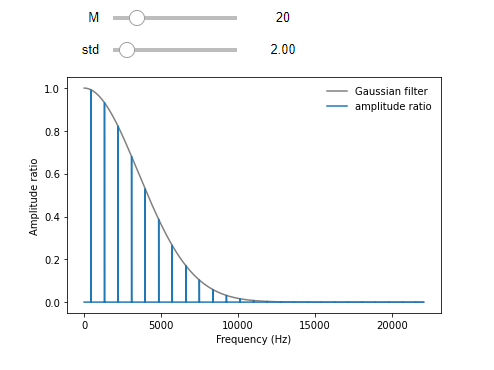
\includegraphics[width=0.8\linewidth]{gauss_20_2}
        \caption{\texttt{m} = 20, \texttt{std} = 2}
        \label{fig:gauss_20_2}
    \end{figure}

    \begin{figure}[H]
        \centering
        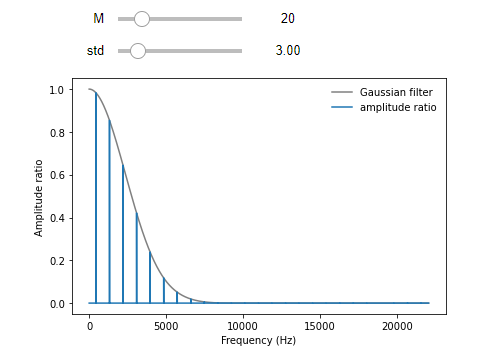
\includegraphics[width=0.8\linewidth]{gauss_20_3}
        \caption{\texttt{m} = 20, \texttt{std} = 3}
        \label{fig:gauss_20_3}
    \end{figure}

    \begin{figure}[H]
        \centering
        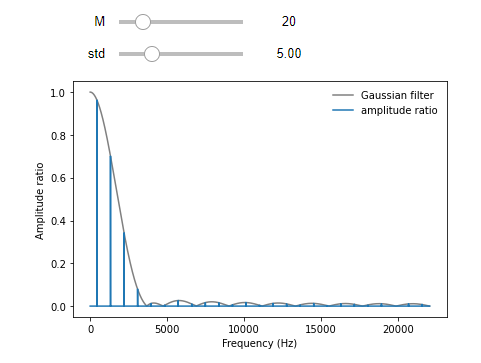
\includegraphics[width=0.8\linewidth]{gauss_20_5}
        \caption{\texttt{m} = 20, \texttt{std} = 5}
        \label{fig:gauss_20_5}
    \end{figure}

    \begin{figure}[H]
        \centering
        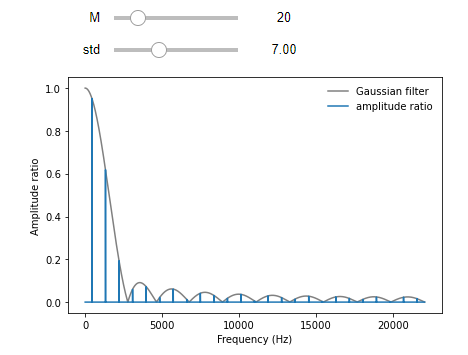
\includegraphics[width=0.8\linewidth]{gauss_20_7}
        \caption{\texttt{m} = 20, \texttt{std} = 7}
        \label{fig:gauss_20_7}
    \end{figure}

    Увеличение \texttt{std} без увеличения \texttt{m} приводит к сплющиванию гауссовой кривой.

    \newpage


    \section{Упражнение №2}
    \label{sec:2}

    В втором упражнении необходимо использовать ДПФ гауссовой кривой на нескольких примерах и понять, что происходит при изменении \texttt{std}.

    Начнем с реализации функции \texttt{plot\_gaussian}, которая будет выводить окно Гаусса и БПФ.

    \begin{lstlisting}[language=Python, caption= Функция plot\_gaussian, label={lst:plot_gaussian}]
        def plot_gaussian(std):
            M = 32
            gaussian = scipy.signal.gaussian(M=M, std=std)
            gaussian /= sum(gaussian)

            plt.subplot(1, 2, 1)
            plt.plot(gaussian)
            decorate(xlabel='Time')

            fft_gaussian = np.fft.fft(gaussian)
            fft_rolled = np.roll(fft_gaussian, M//2)

            plt.subplot(1, 2, 2)
            plt.plot(np.abs(fft_rolled))
            decorate(xlabel='Frequency')
            plt.show()
    \end{lstlisting}

    Реализуем интерактивный виджет для отслеживания изменений.

    \begin{figure}[H]
        \centering
        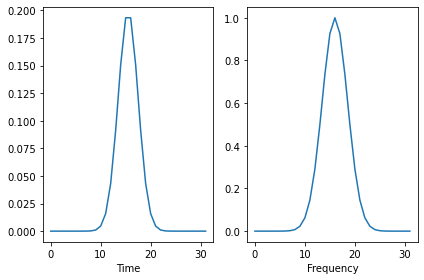
\includegraphics[width=0.8\linewidth]{DTF_2}
        \caption{\texttt{std} = 2}
        \label{fig:DTF_2}
    \end{figure}

    \begin{figure}[H]
        \centering
        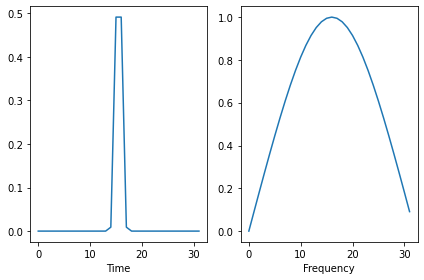
\includegraphics[width=0.8\linewidth]{DTF_0.5}
        \caption{\texttt{std} = 0.5}
        \label{fig:DTF_0.5}
    \end{figure}

    \begin{figure}[H]
        \centering
        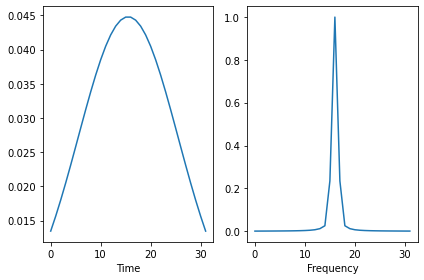
\includegraphics[width=0.8\linewidth]{DTF_10}
        \caption{\texttt{std} = 10}
        \label{fig:DTF_10}
    \end{figure}

    В результате можно сказать, что при увеличении ширины сигнала идет уменьшение преобразования Фурье, и наоборот.

    \newpage


    \section{Упражнение №3}
    \label{sec:3}

    В третьем упражнении необходимо в дополнение к Гауссову окну создать окно Хэмминга тех же размеров.
    Также нужно дополнить окно нулями и напечатать его ДПФ.
    Определить какое окно подходит больше для фильтра низких частот.

    Создадим сигнал для дальнейшей работы.

    \begin{lstlisting}[language=Python, caption= Создание сигнала, label={lst:make_signal}]
        from thinkdsp import SquareSignal

        signal = SquareSignal(freq=440)
        wave = signal.make_wave(duration=1.0, framerate=44100)
    \end{lstlisting}

    Построим нужные окна и выведем их графики.

    \begin{lstlisting}[language=Python, caption= Построение окон, label={lst:make_window}]
        M = 15
        std = 2.5

        gaussian = scipy.signal.gaussian(M=M, std=std)
        bartlett = np.bartlett(M)
        blackman = np.blackman(M)
        hamming = np.hamming(M)
        hanning = np.hanning(M)

        windows = [blackman, gaussian, hanning, hamming]
        names = ['blackman', 'gaussian', 'hanning', 'hamming']

        for window in windows:
            window /= sum(window)

        for window, name in zip(windows, names):
            plt.plot(window, label=name)

        decorate(xlabel='Index')
    \end{lstlisting}

    \begin{figure}[H]
        \centering
        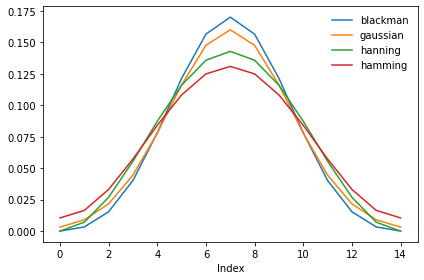
\includegraphics[width=0.8\linewidth]{windows_wave}
        \caption{Графики окон}
        \label{fig:windows_wave}
    \end{figure}

    Графики похожи.

    Дополним окна нулями и выведем их ДПФ.

    \begin{figure}[H]
        \centering
        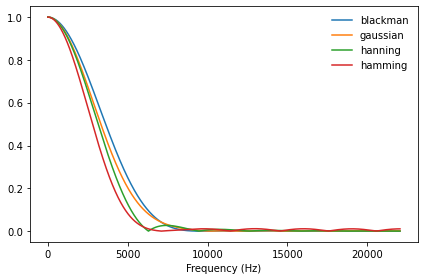
\includegraphics[width=0.8\linewidth]{windows_dtf}
        \caption{ДПФ окон}
        \label{fig:windows_dtf}
    \end{figure}

    По графикам видно, что окно Хэмминга спадает быстрее всех, окно Блэкмана спадает медленнее всех.

    Построим логарифмические графики.

    \begin{figure}[H]
        \centering
        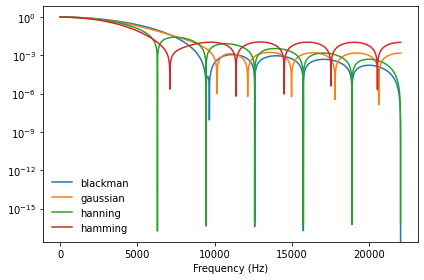
\includegraphics[width=0.8\linewidth]{windows_log}
        \caption{Логарифмический график ДПФ}
        \label{fig:windows_log}
    \end{figure}

    На графиках видно, что сначала значения Хэмминга и Ханнинга падают быстрее, чем два других.

    Из полученных данных можно сделать вывод, что для фильтрации НЧ лучше всего использовать окно Хэмминга, т.к. оно дает меньше "выпуклостей".

    \newpage


    \section{Выводы}
    \label{sec:conclusions}

    В результате выполнения данной лабораторной работы была разобрана зависимость Гауссовой кривой от ширины Гауссового окна.
    Кроме того было установлено, что для фильтрации низких частот лучш всего использовать окно Хэмминга.

\end{document}